\begin{table}[ht]
\centering
\begin{tabular}{llllll}
  \hline
  individual & pch & day1 & day2 & day diff \\ 
  \hline
CB00165D & a & 2012-11-29 & 2013-03-07 & 98 \\ 
CB00366X & b & 2012-11-07 & 2013-03-27 & 140 \\ 
CB00396E & c & 2012-09-25 & 2013-03-11 & 167 \\ 
CB00406Q & d & 2012-10-16 & 2013-01-22 & 98 \\ 
CB01484M & e & 2012-09-25 & 2013-03-11 & 167 \\ 
CB01494Y & f & 2012-10-09 & 2013-01-29 & 112 \\ 
CB01495Z & g & 2012-10-09 & 2013-01-29 & 112 \\ 
CB01498C & h & 2012-10-16 & 2013-01-22 & 98 \\ 
CB01503H & i & 2012-11-07 & 2013-03-07 & 120 \\ 
CB01504J & j & 2012-11-07 & 2013-03-27 & 140 \\ 
   \hline
\end{tabular}
\caption{ \label{figure:recalled-individuals} Individuals recalled beteen 98 and 168 days later. }
\end{table}

In Figure~\ref{figure:channels-doses}, considering the density functions across all channels in resting lymphocytes compared ones stimulated at the highest dose,
there seems to be no need for normalisation since the peaks in the density plots align well.
%normalisation is not required to account for dose effects.
Considering unstimulated lymphocytes across days however, Figure~\ref{figure:channels-days} suggests that there is need for normalisation since the distributions do not always align well.
See for example individual b for marker CD45RA.

\begin{figure}[h]
    \centering
    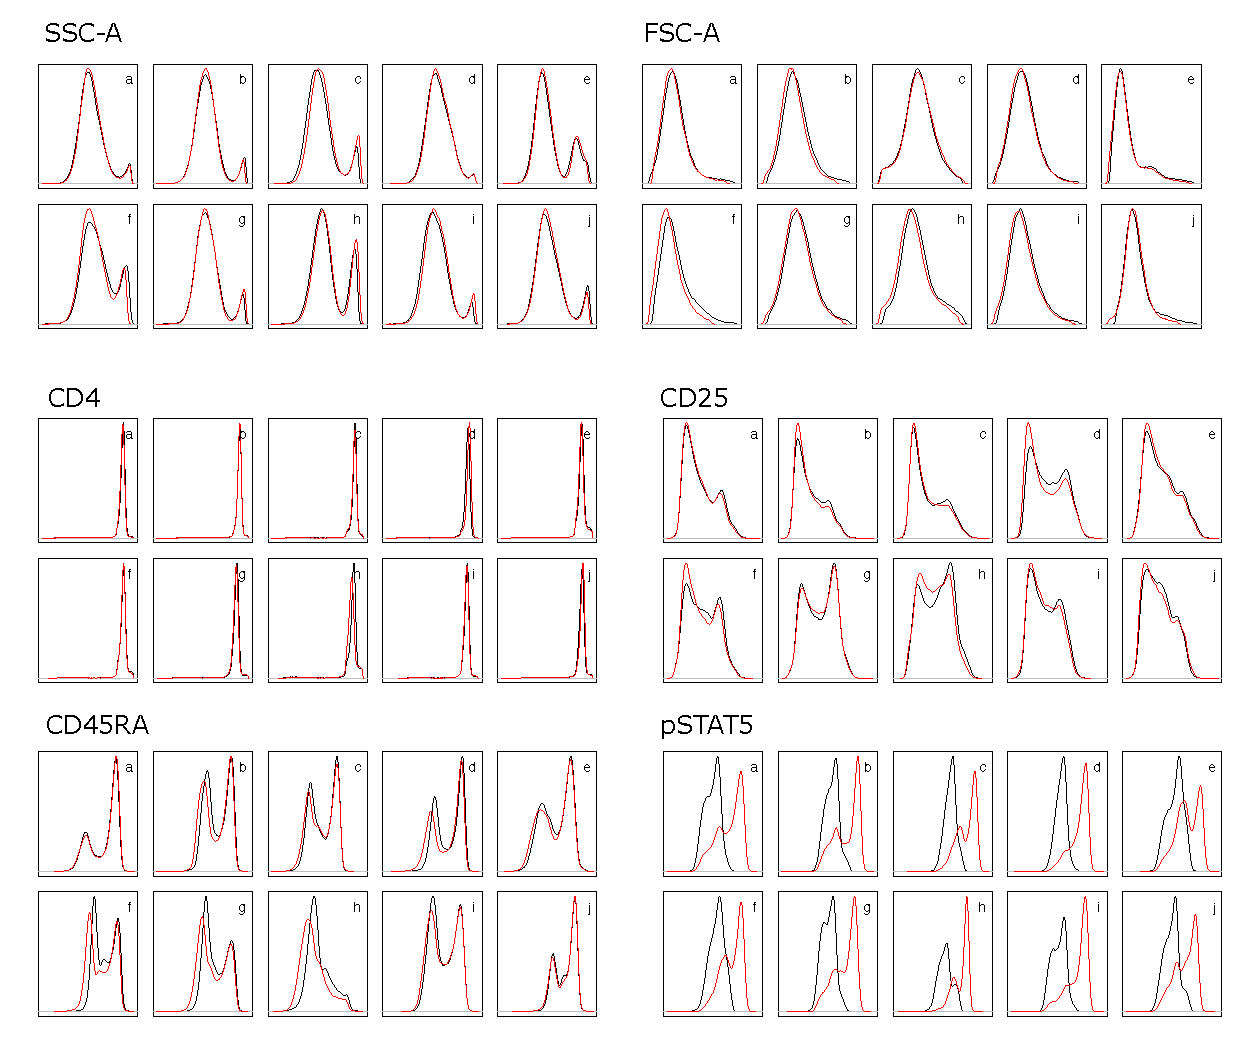
\includegraphics[scale=.75]{IL2/figures/channels-doses.pdf}
    \caption{  \label{figure:channels-doses} 
    In CD4 lymphocytes on same day different doses in 10 individuals (a, b, c, d, e, f, g, h, i, j).
  Black resting doses, in red 1000UL stimulation. As expected as a result of the stimulation, the peak of the pSTAT5 distribution shifts. }
\end{figure}


\begin{figure}[h]
    \centering
    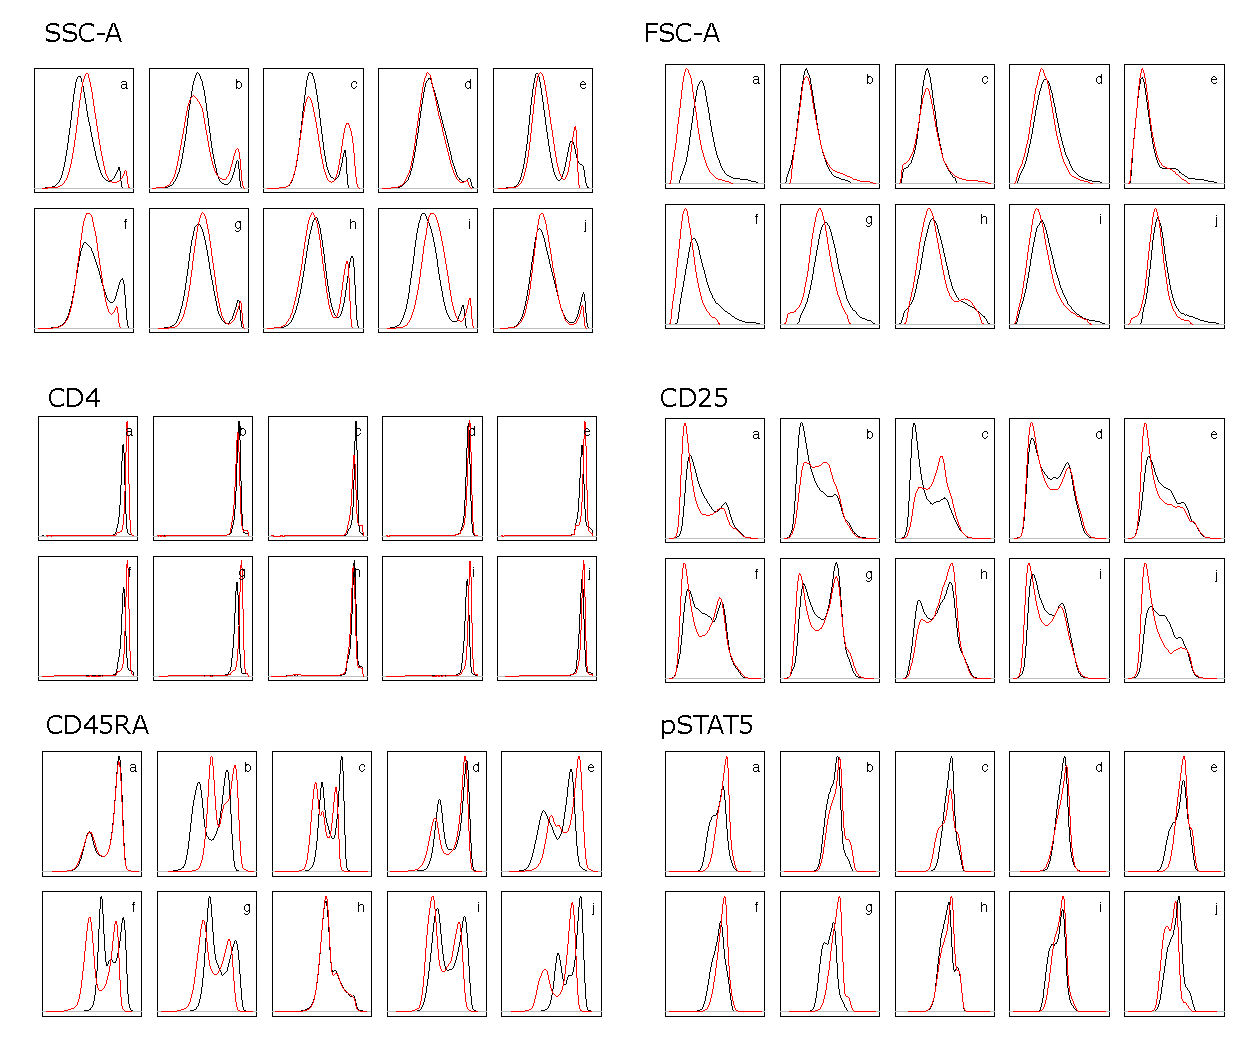
\includegraphics[scale=.75]{IL2/figures/channels-days.pdf}
    \caption{  \label{figure:channels-days} 
    In resting CD4 lymphocytes for each of the 10 individuals (a, b, c, d, e, f, g, h, i, j), black the first day and in red the second day.
    The distributions no longer appear to align as well. This suggests there might be need for normalisation to realign the peaks.}
\end{figure}



%Certain normalisation methods make assumptions about the shape of the data.
%The actual choice of normalisation depends on the characteristics of the data we wish to compare.
%Certain normalisation methods such as quantile normalisation are not appropriate since they assume the distributions have the shame shape.
In the case of flow cytometry data, we expect that the core cell populations should exist in all samples but that their locations and their
proportions may vary across days and \emph{IL-2} dose.
Hence we wish to align the location of the population across days while allowing for the relative proportion of the populations to vary.

\section{Normalisation using Univariate Peak Alignment}

The idea is to identify the groups based on one marker using either a clustering algorithm and then finding the peak to represent the median of the group.
In this approach the number of groups K needs to be known a priori and is assumed to be the same across samples.
This is the method used by \texttt{flowBeads} which identifies groups with the k-medoids algorithm for the purpose of bead normalisation \citep{flowBeads}.
%However peaks are not always easily identifiable.
We also applied this method on qPCR data to align common copy number groups 1 and 2 across plates.

Instead of clustering, another method is to identify peaks in the density function with a sliding window approach.
The sliding window approach records the point with the highest density estimate in the current window.
As a result returning a list of highest density points of which the top K may be chosen.
This is one of the approaches implemented in the flowNorm BioConductor package.
Here's an example of this method applied on simulated data where the number of peaks is known and easily identifiable (Figure~\ref{figure:simulation-peak-align}).

%\begin{figure}[h]
%%
%%#simulated data
%%x0 <- mixtools::rnormmix(1000, mu=c(1,6), lambda=c(.3,.7))
%%x1 <- mixtools::rnormmix(1000, mu=.9*c(1,6)+2, lambda=c(.5,.5), sigma=c(2,2))
%%d0 <- density(x0)
%%d1 <- density(x1)
%%l0 <- extract.landmarks(x0,max.lms=2, bw=d0$bw)
%%l1 <- extract.landmarks(x1,max.lms=2, bw=d1$bw)
%%m <- lm(l0$lms ~ l1$lms)
%%x1.norm <- cbind(1,x1)%*%coefficients(m)
%%l1.norm <- extract.landmarks(x1.norm,max.lms=2)
%%#before align
%%pdf('~nikolas/GoogleDrive/PhD/Thesis/IL2/figures/simulation-peak-align-noise.pdf')
%%plot(d0,xlim=c(-3,11),main='', xlab='')
%%points(l0$lms, l0$dens, pch=20, cex=2)
%%lines(d1, lty=2)
%%points(l1$lms, l1$dens, pch=20, cex=2)
%%#after peak align
%%lines(density(x1.norm), lty=2, col='red')
%%points(l1.norm$lms, l1.norm$dens, pch=20, cex=2, col='red')
%%dev.off()
%%
    %\centering
    %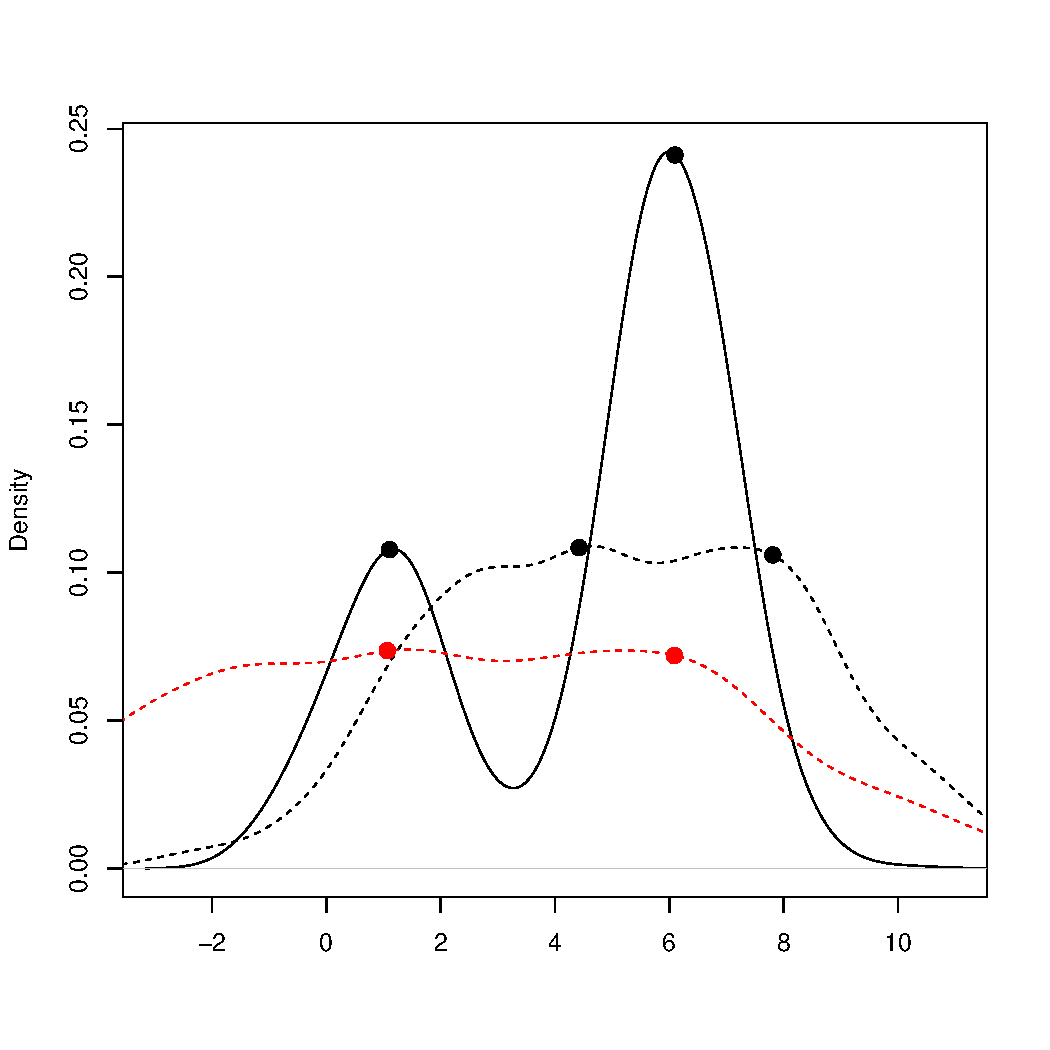
\includegraphics[scale=1]{IL2/figures/simulation-peak-align-noise.pdf}
    %\caption{  \label{figure:simulation-peak-align-noise}  In solid black line represents the density function obtained from $1000$ draws from a mixture of two normal distribution
    %with means $\mu_0=(1,6)$, standard deviations $\sigma_0=(1,1)$ and mixing proportions $\tau_0=(.3,.7)$.
    %The dashed black line represents the density function obtained from $1000$ draws from a mixture of two normal distribution
    %where $\mu_1 = 0.9 \mu_0 + 2$, standard deviations $\sigma_0=(1,1)$ and $\tau_1=(.5,.5)$.
    %The red dashed line represents the transformation using peak alignment. }
%\end{figure}
%



\section{Normalisation of pSTAT5 Response Across Days}


%%e <- lapply(flat.rep.fcs[names(flat.rep.fcs)[1:4]], function(x) ecdf(lgcl(getChannels(x, 'pstat5'))))
%%d <- lapply(flat.rep.fcs[names(flat.rep.fcs)[1:4]], function(x) density(lgcl(getChannels(x, 'pstat5')),bw=.1))
%%d.f <- lapply(d, function(d) splinefun(d$x,d$y))
%%y.max <- max(sapply(d, function(d) d$y)) 
%%e <- lapply(lymph[names(lymph)[1:4]], function(x) ecdf(lgcl(getChannels(x, 'pstat5'))))
%%d <- lapply(lymph[names(lymph)[1:4]], function(x) density(lgcl(getChannels(x, 'pstat5')),bw=.1))
%%d.f <- lapply(d, function(d) splinefun(d$x,d$y))
%%y.max <- max(sapply(d, function(d) d$y)) 
%%#pdf('~nikolas/lymph-dose-effect.pdf',width=10,height=5)
%%pdf('~nikolas/ungated-dose-effect.pdf',width=10,height=5)
%%par(mfrow=c(1,2))
%%x <- seq(-.5, 3, length.out=20000)
%%plot(x, e[[1]](x), col='white', xlab='pSTAT5', xlim=c(-.5,3), ylab='') 
%%mapply(function(e,lwd,lty) lines(x,e(x),lwd=lwd,lty=lty),e,seq(1,2.5,.5),c(1,2,2,1))
%%legend('topleft',doses, lwd=seq(1,2.5,.5), lty=c(1,2,2,1))
%%plot(x, d.f[[1]](x), col='white', xlab='pSTAT5', xlim=c(-.5,3),ylim=c(0,1),ylab='') 
%%mapply(function(d,lwd,lty) lines(x,d(x),lwd=lwd,lty=lty),d.f,seq(1,2.5,.5),c(1,2,2,1))
%%legend('topleft',doses, lwd=seq(1,2.5,.5), lty=c(1,2,2,1))
%%dev.off() 
%%pdf('~nikolas/ungated-lymph-dose-effect.pdf')
%%par(mfrow=c(1,1))
%%x <- seq(-.5, 3, length.out=20000)
%%plot(x, d.f[[1]](x), col='white', xlab='pSTAT5', xlim=c(-.5,3),ylim=c(0,1),ylab='') 
%%d <- lapply(flat.rep.fcs[names(flat.rep.fcs)[c(1,4)]], function(x) density(lgcl(getChannels(x, 'pstat5')),bw=.1))
%%d.f <- lapply(d, function(d) splinefun(d$x,d$y))
%%y.max <- max(sapply(d, function(d) d$y))
%%mapply(function(d,lwd,lty) lines(x,d(x),lwd=lwd,lty=lty),d.f,c(1,2.5),1)
%%d <- lapply(lymph[names(lymph)[c(1,4)]], function(x) density(lgcl(getChannels(x, 'pstat5')),bw=.1))
%%d.f <- lapply(d, function(d) splinefun(d$x,d$y))
%%y.max <- max(sapply(d, function(d) d$y))
%%#r <- mapply(function(a,b) length(a)/length(b), lymph[1:4], flat.rep.fcs[1:4])
%%mapply(function(d,lwd,lty) lines(x,d(x),lwd=lwd,lty=lty,col='red'),d.f,c(1,2.5),1) 
%%legend('topleft',doses[c(1,4)], lwd=c(1,2.5), lty=1)
%%dev.off()
%%lymph <- sapply(flat.rep.fcs, function(x) { cd4 <- lgcl(getChannels(x, 'cd4')); return(x[2 <  cd4 & cd4 < 2.75,]) })
%%


\begin{figure}[h]
    \centering
    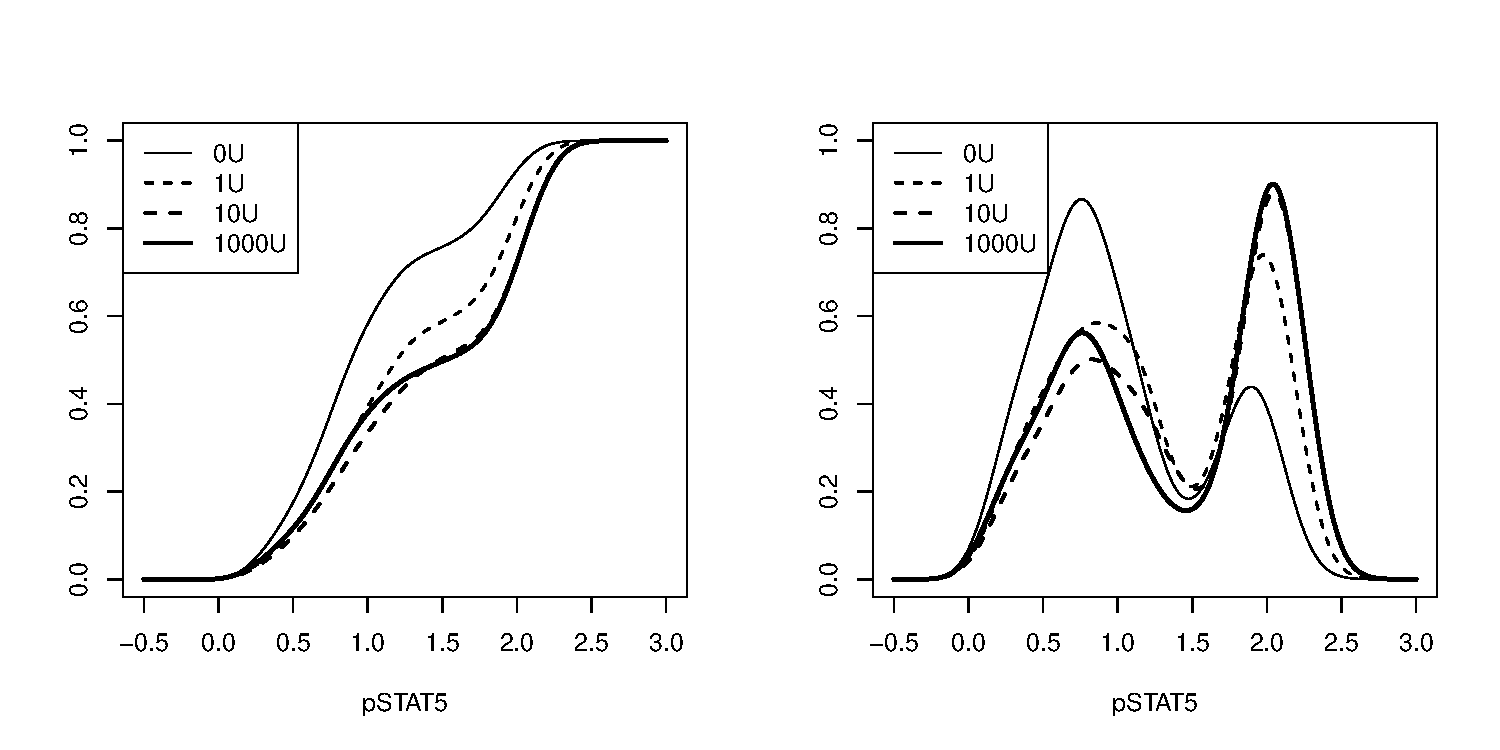
\includegraphics[scale=.5]{IL2/figures/ungated-dose-effect.pdf}
    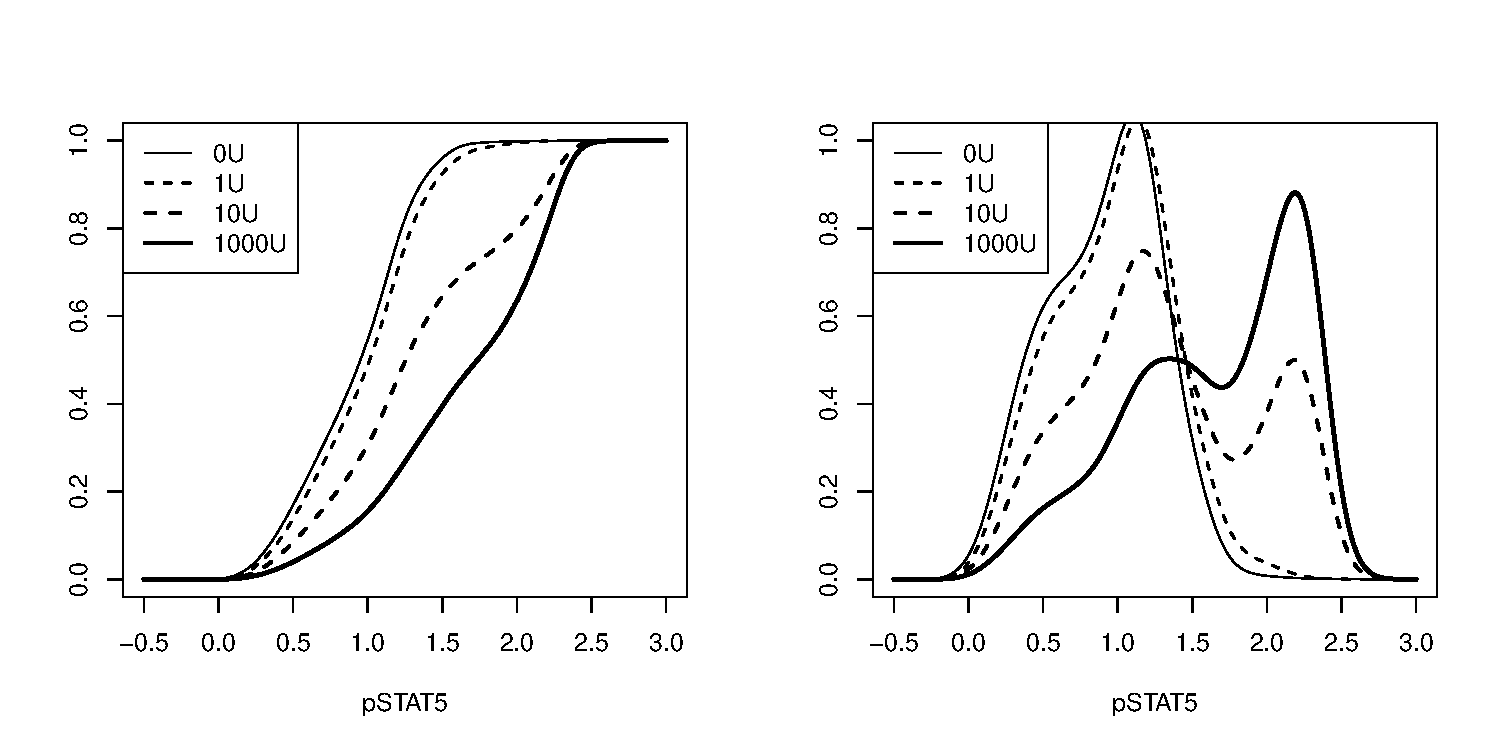
\includegraphics[scale=.5]{IL2/figures/lymph-dose-effect.pdf}
    \caption{  \label{figure:dose-effect}
        On the left the cumulative density function obtained from individual a on day 1 across 4 increasing doses.
        On the right the density function.
        The top two figures are from the ungated sample.
        The bottom two figures are from a CD4 range gate.
        We observe that in the unstimulated sample the distribution is already bimodal 
        and that upon stimulation the location of the peaks does not change much but that the height changes greatly.
        Contrary to the ungated data, the pSTAT5 distribution in the CD4 gated sample now appears unimodal when resting or stimulated
        at the lowest 1U dose.  At the higher doses we start seeing a bimodal distribution.
        In the ungated sample, the location of the activation peak seems to align somewhat with that of the activation peak.  }
\end{figure}

Another method is to not concern ourselves with aligning the cell populations but instead to focus on the reproducibility of the response in terms of relative shift in the pSTAT5 distribution
across days in various cell populations.
The idea being that unstimulated sample should yield the baseline on that day.



The relative shift in the pSTAT5 distribution between resting and stimulated can be measured by computing the area between the cumulative density functions of the unstimulated and stimulated samples.

In Figure~\ref{figure:dose-effect} we observe that the dose effect is very different in the ungated than in the CD4 gated subset (lymphocytes) which represent around $10\%$ of
the whole sample.
The lowest 1U dose seems to have a much more stronger relative effect in the whole sample than in the lymphocyte subset which suggest that there sizeable amount of cells in the ungated
data which are much more sensitive to low doses of IL-2 than the lymphocytes.
However the relative difference in response between 10U and 1000U seems much more important in lymphocytes than in the whole sample
Also since the resting sample sample display a shoulder in resting state it seems that lymphocytes even in a resting state are a mixture of resting and semi-activated lymphocytes.


Given that the location of the peaks of pSTAT5 remain stable but that the heights vary in the ungated sample this advocates a normalisation method which relies on peak alignment.


In the manual analysis conducted by Tony Cutler, he found that he could identify individuals which were low or high responders.
This leads us to hypothesise that within one individual the response to \emph{IL-2} on day 1 should be comparable to the response to \emph{IL-2} on day 2.

%One method we have tried is based on the assumption is that in the ungated data, the bottom and top percentile of the pSTAT5 distribution do not respond to \emph{IL-2} and so can be used as reference points.  This is effectively a quantile normalisation method aligning the bottom and top percentile across doses.

%However we found that this normalisation method d is not true in CD4+ lymphocyte gated data.


